\documentclass[12pt]{article}
\usepackage[utf8]{inputenc}
\usepackage[frenchb]{babel}
\RequirePackage[usenames,dvipsnames,xcolor=pst]{pstricks}
\RequirePackage{epsfig} % for eps fig
\RequirePackage{pst-blur} % for nice shadow
\RequirePackage{pst-dbicons} % for E/R
%\RequirePackage{mon-pst-uml} % for my own UML package
\RequirePackage{pst-uml} % for my own UML package
\RequirePackage{tikz} % circles such as History pseudostate
\newcommand{\monpsgrid}{\psgrid}
%\newcommand{\monpsgrid}{}
\setlength{\topmargin}{-5mm}%
\setlength{\oddsidemargin}{-1mm}%
\setlength{\evensidemargin}{-1mm}%
\setlength{\textwidth}{15.5cm}%
\setlength{\textheight}{8.9in}%
%------------------------------------
%   QCM
%------------------------------------
%\usepackage[french,correction]{qcm} % to print correct answers
%\usepackage[french]{qcm}
\title{\vspace{-3pc}\textbf{Contr\^ole M2105 (S2 -- 	IHM)}}

\date{lundi 9 mars 2015 -- Une seule feuille A4 manuscrite autoris\'ee\\
Dur\'ee : 1h00}

\def\dc{\textsf{diagramme de classe}}
\def\sni{\textsf{SNI}}
%===========================================================
\begin{document}
\maketitle

\begin{center}
\fbox{
  \begin{minipage}{6in}
    Nom : ~~~~~~~~~~~~~~~~~~~~~~~~~~~~~~~~~~~~~~~~~~~ Prénom : \\
  \end{minipage}
}
\end{center}

\section{Ecrire un SNI}

\subsection{Construction classique}

\subsection*{Sujet}

Une banque souhaite réaliser une application interactive de gestion des clients
et des comptes pour mettre à la disposition des employés et des chefs d'agences.
Une étude des besoins montre que chaque client peut posséder plusieurs comptes.
Chaque compte est  identifié par un numéro et possède un certain type
(Courant, Epargne, Epargne logement, Etudiant, Livret, \ldots).
Chaque compte comporte des opérations qui ont aussi un certain type
(Dépôt de chèque, Dépôt de liquide, Retrait GAB, Retrait au guichet, Virement,
\ldots). Si le montant de l'opération est positif il s'agit d'un crédit, s'il
est négatif c'est un débit.
Si le solde d'un compte est négatif c'est qu'il est à découvert. Ce découvert
ne doit pas dépasser le découvert autorisé qui est spécifique de chaque compte.
Les fonctions suivantes ont été demandées par les utilisateurs :
\begin{enumerate}
\item Afficher le détail d'un compte à partir de son numéro saisi au clavier. Le détail du compte fera apparaître le code et le nom du client, le numéro de compte, le type de compte, le solde actuel et le découvert autorisé.
\item Afficher les opérations d'un compte à partir du détail du compte. Chaque opération fera apparaître une date, un libellé, un montant (positif ou négatif) et le type d'opération.
\item Saisir une opération concernant un compte en vérifiant que le compte ne dépasse pas le découvert autorisé s'il s'agit d'une opération de débit.
\item Afficher la liste de tous les clients faisant apparaître simplement le code et le nom de chaque client puis, en sélectionnant un client dans la liste, afficher le détail du client (codeClient, nom, adresse, téléphone, courriel).
\item A partir d'un client affiché on pourra modifier toutes ses données sauf son code.
\item Saisir un nouveau compte pour un client donné (seuls le numéro, le type de compte et le découvert autorisé sont saisis, le solde est automatiquement mis à zéro).
\item Afficher la liste des comptes débiteurs (numéro et solde) et pouvoir imprimer la liste comportant en plus le nom du client.
\item Editer un courrier à plusieurs clients débiteurs sélectionnés dans la liste pour leur demander d'approvisionner leur compte.
\end{enumerate}

\subsection*{Question}

Réalisez un \sni{} intégrant un maximum de fonctionnalité.

\begin{center}
\fbox{
  \begin{minipage}{6in}
    \hfill\vspace{6in}
  \end{minipage}
}
\end{center}

\subsection{Générateur automatique}

\subsection*{Question}

\`A partir du \dc{} suivant (\copyright{} Christian Soutou, enseignant de R\&T), et en vous inspirant de la technique de
 construction structurée OBJET-ACTION vue en cours, réalisez un
 \sni{} correspondant (sans trop se soucier des noms des menus).

\begin{center}
\scalebox{0.2}{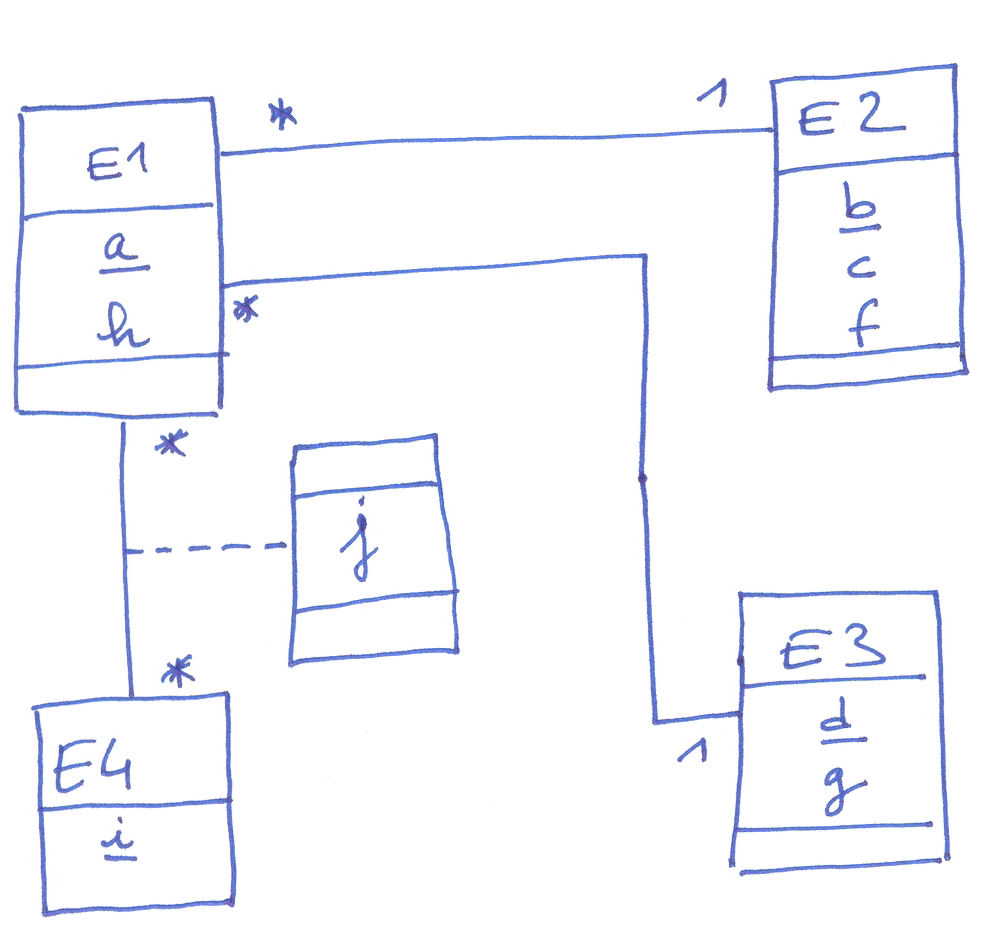
\includegraphics{images/Soutou.jpg}}
\end{center}

\begin{center}
\fbox{
  \begin{minipage}{6in}
    \hfill\vspace{4.5in}
  \end{minipage}
}
\end{center}

\section{Diagramme de classe et SNI}

\subsection{Diagramme de classe à partir d'un SNI}

\subsubsection*{Botoutou}

Soit le \sni{} suivant, représentant l'interface souhaitée par la clinique vétérinaire ``Botoutou" :

\begin{center}
\scalebox{0.8}{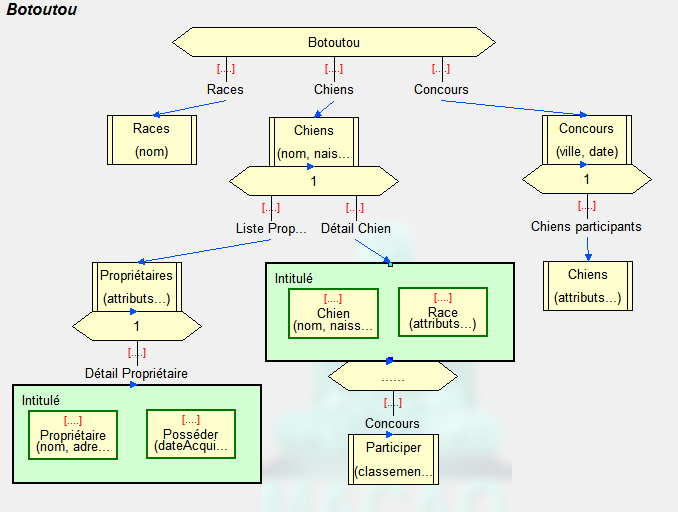
\includegraphics{images/SNI-Botoutou.png}}
\end{center}

\subsubsection*{Question}

Réalisez un \dc{} respectant ce \sni. Celui-ci ne comportera \textbf{que} des éléments déduits du \dc.
D'ailleurs vous pourrez numéroter chaque élément de votre diagramme et proposer une légende pour chacun
de ces éléments, à la suite de votre diagramme, qui précise la justification de cet élément.

\begin{center}
\fbox{
  \begin{minipage}{6in}
    \hfill\vspace{5in}
  \end{minipage}
}
\end{center}

\subsection{Diagramme de classe du SNI}

\subsubsection*{Question}

Réalisez un \dc{} représentant les différents concepts
d'un \sni{} et leurs relations entre eux.
Essayez d'être le plus exhaustif possible mais surtout d'avoir
un \dc{} correct.

On pourra s'inspirer du début de diagramme suivant :

\begin{center}
\scalebox{0.5}{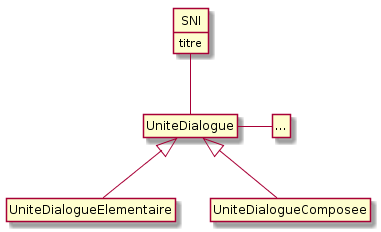
\includegraphics{images/sni.png}}
\end{center}

\begin{center}
\fbox{
  \begin{minipage}{6in}
    \hfill\vspace{5in}
  \end{minipage}
}
\end{center}

\section{Définitions}

\subsection*{Donnez les définitions des termes suivants (une ou deux phrases)}

\subsubsection*{SNI}

\fbox{ \begin{minipage}{6in} \hfill\vspace{1.5in} \end{minipage} }


\subsubsection*{Mode Esquisse (pour la construction d'un SNI)}

\fbox{ \begin{minipage}{6in} \hfill\vspace{1.5in} \end{minipage} }

\subsubsection*{GUI}

\fbox{ \begin{minipage}{6in} \hfill\vspace{1.5in} \end{minipage} }

\subsubsection*{Filtre}

\fbox{ \begin{minipage}{6in} \hfill\vspace{1.5in} \end{minipage} }

\section*{Bar\`eme prévisionnel}

\begin{description}
\item[1.1] 5 points
\item[1.1] 3 points
\item[2] 3 points
\item[3] 4 points
\item[4] 4 points
\item[Propret\'e]  1 point
\end{description}

\end{document}
%===========================================================
